\section{\Glsfmtlong{asr}}

Le modèle d'\gls{asr} permet de transformer la parole aphasique en texte
dans le but de l'utiliser comme entrée pour le modèle de traduction.
Les étapes de sa construction sont établies dans la section précédente.
Dans cette section, nous allons détailler ces étapes.

\subsection{Préparation des données}

La première étape de tout projet de \gls{ml} est la préparation des données.
Dans ce cas, le jeu de données doit être constitué de couples de morceaux d'audio et de leurs transcriptions textuelles.

\subsubsection{Choix du corpus et collecte de données existantes}

\begin{wrapfigure}{r}{2cm}
    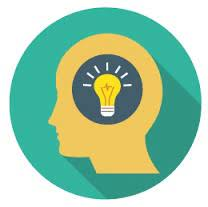
\includegraphics[width=1.5cm]{assets/images/bank.jpeg}
    \caption*{\footnotesize AphasiaBank.}
\end{wrapfigure}

Notre choix s'est porté sur le corpus \textit{AphasiaBank}~\cite{MacWhinney_Fromm_Forbes_Holland_2011}.
Il fait partie du projet \textit{TalkBank}~\cite{macwhinney2007talkbank},
une collection de bases de données créées pour l'étude du langage.
AphasiaBank contient plusieurs vidéos d'entre-teints entre des chercheurs 
et des personnes souffrant de l'aphasie de Broca.
Ses vidéos sont accompagnées par des transcriptions textuelles faites par des experts dans un format particulier.
La qualité des transcriptions est donc excellente.

Cependant, le volume de données sur l'aphasie de Broca est très limité.
En effet, un seul des 11 exemples disponibles en français est un exemple de l'aphasie de Broca.
Il s'agit d'une vidéo de 12 min 03 s, qui contient 3000 mots.
Il faut noter que la moitié de ces mots sont prononcés par le chercheur.
La durée effective de la parole aphasique est donc de 6 min.
Cela est de très loin insuffisant pour entraîner un modèle profond.
Pour ce but, il est nécessaire de collecter des données supplémentaires. 

\subsubsection{Collecte de données supplémentaires}

Les données d'AphasiaBank étant insuffisantes, d'autres sources sont nécessaires.
Plusieurs enregistrements de personnes souffrant de l'aphasie de Broca sont disponibles sur internet 
(YouTube, Vimeo, \dots).
La qualité de ces enregistrements est très variable et largement inférieure à celle d'AphasiaBank.
Cependant, leur ajout au corpus est nécessaire pour augmenter sa taille.

Notre recherche nous a permis d'obtenir 22 enregistrements de personnes souffrant de l'aphasie de Broca 
d'une durée totale de 48 min 44 s.
Des statistiques sur la répartition démographique de ces enregistrements 
sont présentées dans le tableau~\ref{tab.asr-data-demographics}.
\begin{table}[hbt]
    \begin{center}
        \begin{tabular}{|l|c|c|}
            \cline{2-3}
            \multicolumn{1}{c|}{}& \textbf{Nombre}& \textbf{Durée}\\
            \hline
            Hommes               & 7              & 13 min 45 s   \\
            \hline
            Femmes               & 31             & 34 min 2 s    \\
            \hline
            Groupe               & 2              & 9 min 57 s    \\
            \hline
        \end{tabular}
    \end{center}
    \caption{Répartition des enregistrements collectés par genre.}
    \label{tab.asr-data-demographics}
\end{table}
On y observe que les enregistrements sont assez diverses en comparaisons l'unique enregistrement trouvé sur AphasiaBank.

\subsubsection{Transcription et filtrage des données}

Les 22 enregistrements collectés sont transcrits à l'aide de 
Whisper~\cite{Radford_Kim_Xu_Brockman_McLeavey_Sutskever_2022}.
Cela permet d'avoir des transcriptions textuelles de qualité.
Cependant, les transcriptions obtenues contiennent des erreurs (particulièrement pour les prononciations aphasiques).

L'étape suivante est donc de filtrer à la main les transcriptions obtenues.
Cela permet de corriger les erreurs de transcription 
et de réintroduire les prononciations aphasiques éliminées par Whisper.
La sortie de cette étape est un corpus (parole/écrit).

Les données d'AphasiaBank sont déjà transcrits, mais cela est fait dans un format particulier.
Il est donc nécessaire de réécrire les transcriptions en français standard.
L'exemple d'AphasiaBank et donc ajouté au corpus, ce qui fait un total de 1 h 0 min 47 s de parole aphasique.
Cela est encore insuffisant pour entraîner un modèle profond.
Cependant, il peut servir aux chercheurs qui souhaitent travailler sur l'aphasie de Broca.
On rend donc disponible ce corpus.

\subsection{Création et entraînement du modèle}

Les données collectées n'étant pas suffisantes,
il n'est pas possible d'entraîner un modèle de \gls{dl}.
Nous avons donc décidé de mettre en pause le développement de ce modèle 
jusqu'à ce que des données supplémentaires soient disponibles.

Dans le but de faciliter l'accès à de telles données,
nous avons mis notre corpus à la disposition des chercheurs.
Pour le reste de ce projet,
nous nous focalisons sur le modèle de traduction.